\documentclass{seal_article}
\usepackage{seal}
\usepackage{longtable}
\usepackage{xcolor}
\usepackage{graphicx}

\iftexshop
\usepackage{pdfsync}
\fi

\title{FeedBag Dashboard}
\subtitle{Master Project}

\begin{document}
\maketitle

\iftexshop
\setprotcode\font
{\it \setprotcode \font}
{\bf \setprotcode \font}
{\bf \it \setprotcode \font}
\pdfprotrudechars=2
\fi

\noindent Master Project\\
\noindent Project period\\
\noindent Severin Siffert \newline severin.siffert@uzh.ch \newline Timothy Zemp \newline timothy.zemp@uzh.ch \newline Sarah Zurmühle \newline sarah.zurmuehle2@uzh.ch\\
\noindent Sebastian Proksch

\section{Introduction}
Microsoft’s Visual Studio\footnote{​https://visualstudio.microsoft.com} is an IDE for software developers. It makes the task of programming easier and faster. However, it is not possible to track your own interactions on the IDE itself. Showing developers e.g. how much time they spend on testing or debugging can help them analyzing and improving their work. Dr.-Ing. Sebastian Proksch has developed, in the scope of the ​KaVE Project\footnote{​http://www.kave.cc/home}, an interaction tracking extension for Visual Studio called ​FeedBag\footnote{ ​http://www.kave.cc/feedbag}. This tool tracks mostly all interactions performed on Visual Studio. Developers have access to their own collected data and they have the possibility to submit it to the KaVE team for their researches.

The FeedBag project is not completed yet. Browsing through the collected data and trying to find a pattern is an arduous task and it is not suited for developers which have not much time in their hand. There exists no convenient way yet to show statistics of the data to the users.

If the users do not see any significant benefit from sharing their data, they will mostly not use FeedBag. However, if they can get an advantage, we belief that more users will get motivated to use the tool. Furthermore, if the privacy setting will get enhanced, possible users will feel safer using FeedBag. One goal of our project is to make FeedBag more useful for the users, but another goal is to increase the data collection process. With more users, the collected data from the FeedBag extension will increase and the KaVE research team will have more resources for their research.

Therefore, in the scope of our master project, we work on an extension of FeedBag. We will create a dashboard which visualizes relevant information generated by the collected data from Visual Studio. We will firstly find out what kind of information is useful for our users, generate visualizations, test their effectiveness, handle the data analyzation and privacy issues and lastly integrate everything together. Our dashboard is not only a highly relevant part of making FeedBag useful to the software developer community, it also set a starting stone for further development and research in this kind of field. Therefore, we are convinced that our dashboard will be further enhanced in the future outside of our master project scope.

\section{Project Description}

\subsection{Overview}
\subsection{Scope of the work}
\subsection{Intended results}

\section{Related Work}
While there exists a lot of literature about organizational productivity, there is very little research about individual developers’ productivity and self-monitoring to improve personal skill and productivity. What little research exists ​\cite{Meyer:2014:SDP:2635868.2635892, Meyer:2017:DRS:3171581.3134714} agrees that the number and size of completed tasks is the biggest indicator of productivity, but does not suffice by any means. The completed tasks should be accompanied by high-level overviews as well as fine-grained details, the subject of which highly depend on the individual.

Conducted surveys ​\cite{Meyer:2014:SDP:2635868.2635892, Meyer:2017:DRS:3171581.3134714} indicate that making measurements about their day will make a significant amount of developers reflect on poor habits and do their best to implement change. Since no study really defined what productivity means, no conclusions were drawn about how big the actual improvements were, both in short as well as long term.

The biggest issues identified with self-monitoring in Meyer et al.'s study \cite{Meyer:2017:DRS:3171581.3134714} were as follows: Oftentimes, the tools available do not serve the users’ requirements very well. One major pain point was lacking context information, because many tools only cover a narrow spectrum of activities and leave out entire sections relevant to the task, such as ignoring anything related with email or informal meetings. Even when enough data was available, people still have trouble identifying and interpreting interesting data and turning it into actionable advice for themselves. Also, users reported that simple stated statistics, delivered in natural language (example: “You tend to be more productive in the afternoon”) had the best results in enabling them to change their behaviour. The last major pain point are concerns about privacy, such as the data being misused or getting into a bosses’ hands who then will draw bad conclusions are a big showstopper for a sizeable chunk of the population.

Experience Sampling turned out to be very effective to foster change \cite{Meyer:2017:DRS:3171581.3134714}. Experience Sampling occurs when a pop-up occasionally asks about the current productivity level. A recommended interval according to Meyer et al. \cite{Meyer:2017:DRS:3171581.3134714} is every hour. The authors speculate that the positive influence comes from the fact that the current level of productivity is very hard to asses automatically and because the pop-up forces the programmers to do some self-reflection, which helps them staying focussed on what they are trying to achieve.


\section{Background Material}

\subsection{Why a dashboard?}
Meyer et al. \cite{Meyer:2017:DRS:3171581.3134714} stated, that there are three important points one has to consider when building a soft-monitoring tool for a workplace: 
\begin{enumerate}
	\item the varied need of the users have to be met in the data collection and representation step
	\item it should be possible for the users to actively engage with the system
	\item the tool should provide more insights into the users work
\end{enumerate}
To fulfil all these requirements, creating a dashboard which can be adapted freely to the users needs and let the users interact with the tool, seems to be the best solution for our use case. 

\subsection{Useful Productivity Measures}
	In 2014 Meyer et al. \cite{Meyer:2014:SDP:2635868.2635892} conducted a survey to find out what activities software developers think of as productive. As part of their research, they ask developers which measurements would help them to assess their personal productivity. The following 23 measures were their result: 
	\begin{itemize}
		\item Number of closed work items (tasks and bugs)
		\item Spend time on each work item
		\item Spend time reviewing code.
		\item Spend time writing code.
		\item Number of contributed code reviews
		\item Number of created work items which were fixed 
		\item Number of created work items
		\item Spend time in meetings
		\item Number of signed off code reviews
		\item Number of written test cases
		\item Spend time on web browsing for work related information
		\item Number of attended meetings
		\item Average time for signing off on code reviews
		\item Spend time in each code project or package
		\item Number of written test cases which afterwards failed
		\item Average time to respond to emails
		\item Spend time on web browsing during work for personal matters
		\item Number of learned API methods each day
		\item Number of commits
		\item Number of written emails
		\item Number of changed lines of code per day
		\item Number of changed code elements for the first time
	\end{itemize} 
	These measures give us a good overview about what developers think can help them improve their own productivity. However, they are not all applicable for our dashboard. For instance, we cannot measure how much time the developers spend in meetings nor can we measure activities outside of Visual Studio (e.g. the time spend on writing emails). Therefore, we selected the measures of Meyer et al.'s findings \cite{Meyer:2014:SDP:2635868.2635892} which were the most relevant for our project:
	\begin{itemize}
		\item Spend time on each work item (coding, testing and debugging)
		\item Spend time reviewing code.
		\item Spend time writing code.
		\item Number of created work items
		\item Number of signed off code reviews
		\item Number of written test cases
		\item Average time for signing off on code reviews
		\item Spend time in each code project or package
		\item Number of written test cases which afterwards failed
		\item Number of commits
		\item Number of changed lines of code per day
	\end{itemize}
	In 2017, Meyer et al. \cite{Meyer:2017:DRS:3171581.3134714} designed recommendations for self-monitoring in the workspace. For their study, they ask developers to rate how interesting some metrics would be to reflect on their work day or work week. There were some metrics, which are unsuitable for our study, so we picked the ones which can be implemented in our dashboard:
	\begin{itemize}
		\item Spend time on each file
		\item Spend time on each Visual Studio project
		\item Number of looked at or edited code files
		\item \textcolor{blue}{Spend time writing code}
		\item \textcolor{blue}{Number of done code reviews}
		\item \textcolor{blue}{Spend time on code reviews}
		\item \textcolor{blue}{Number of commits}
		\item Commit size
		\item \textcolor{blue}{Spend time on testing and debugging}
	\end{itemize}
	The blue entries are also appearing in the findings of Meyer et al. \cite{Meyer:2014:SDP:2635868.2635892} which gives them even more creditability. 
	According to the combined findings of Meyer et al. \cite{Meyer:2014:SDP:2635868.2635892} and Meyer et al. \cite{Meyer:2017:DRS:3171581.3134714} we conclude that it would be the most efficient to include time and quantitative measures in our dashboard. Therefore, visualising time intervals, timelines or histograms might be an effective way to visualise our metrics.\\
	
	However, we cannot count only on tracking numbers. As Treude et al. \cite{Treude:2015:SMD:2786805.2786827} stated, you cannot track all facets of development activities with only numbers. Metrics like number of code written per hour are not widely accepted. A textual summary of activities is another alternative to simply presenting numbers. With textual summaries it is possible to explain an activity rather than only measuring an activity. It provides the chance to include individual user-specific context. It would be ideal, to combine textual summaries with measured numbers \cite{Treude:2015:SMD:2786805.2786827}. For now it is not clear how we intent to include these findings in our dashboard, but we will keep them in mind.
	
	Beller et al. \cite{Beller:2016:CEW:2897022.2897027} analyzed the WatchDog tool, which tracks the developers testing activities. Similarly to our project, WatchDog presents the users testing activities as bar- and pie-charts. Additionaly, WatchDog generates a project report, which includes all tracked statistics. The project report does not only inlcude the values of the respective user, but also the average value of all users. This enables the user to compare their own results to the average. 
	
	Combining the findings from Treude et al. \cite{Treude:2015:SMD:2786805.2786827} and Beller et al. \cite{Beller:2016:CEW:2897022.2897027} we are convinced that if we additionally including some textual summaries or reports, it would benefit our dashboard. 
	
\subsection{Dashboard Design}

Meyer et al. \cite{Meyer:2017:DRS:3171581.3134714} defined six tool design recommendations for helping developers increasing their productivity:
\begin{enumerate}
	\item "High-level overviews and interactive features to drill- down into details best support retrospecting on work
	\item Interest in a large and diverse set of measurements and correlations within the data
	\item Experience sampling increases the self-awareness and leads to richer insights
	\item Reflecting using the retrospection creates new insights and helps to sort-out misconceptions
	\item Natural language insights are useful to understand multi-faceted correlations
	\item Insights need to be concrete and actionable to foster behaviour change" \cite[p. 2]{Meyer:2017:DRS:3171581.3134714}
\end{enumerate}
For our project, recommendation 2 and 5 are important. It is interesting, that developers prefer correlating data. We implemented this aspect by correlating time with quantity. Furthermore, we were surprised, that visualisations are not as clear to every developer than we thought. We kept this piece of information in mind while designing our graphics. 

\section{Project Management}

\subsection{Objectives and priorities}
The FeedBag dashboard should be an extension to the Feedback-Ecosystem. However, not everything should be included inside the IDE. The option of sharing the user’s data should still be accessible inside Visual Studio, however, if the user wishes to get access to our dashboard, it should be opened inside the user’s home browser.

To better define our goals, we split the structure of our project in three parts: Data Collection, Backend and Frontend. In the following subsections, we will describe our goals for these separate structure parts. Figure \ref{fig:struct} presents an overview of the structure of our FeedBag dashboard.

\subsubsection{Data Collection}
The Data Collection part consist of the already included data collection features of FeedBag. However, we plan to research about the privacy concerns of using these data. With the GDPR, which got active in Mai 2018, developers have to rethink how they are going to comply to the new privacy protection law. So, one goal of our project is to adapt the already existing data collection process to these new norms.

\subsubsection{Backend}
The next goal consists of generating clean data from the raw data which results from the Data Collection part. However, it is not clear yet if a cleanup is necessary. If we see in a later stage of our project that it is in fact necessary, Dr. Proksch is going to implement the data cleaning for us.

The main goal of the Backend part is to create one (or multiple) so called Processor which is responsible for processing the new data into a form which can be used later in the Frontend part (see next subsection) without reprocessing all data from scratch with every update.

\subsubsection{Frontend}
The Frontend part consists of the visualisation of graphics and statistics of the user’s data. One goal is to find out, what kind of information is important for our users. We will research about the software developer community and try to find out which piece of information about developers coding behaviour is most valuable and helpful.

The data which was processed in the Processor part has to be transformed into JSON in order to use it on the web page. The next goal is to create easy to understand graphics using the JSON data. The webpage has finally to be linked to the FeedBag extension in Visual Studio, so that the user can easily access it.

\subsection{Project steps}
\begin{figure}
  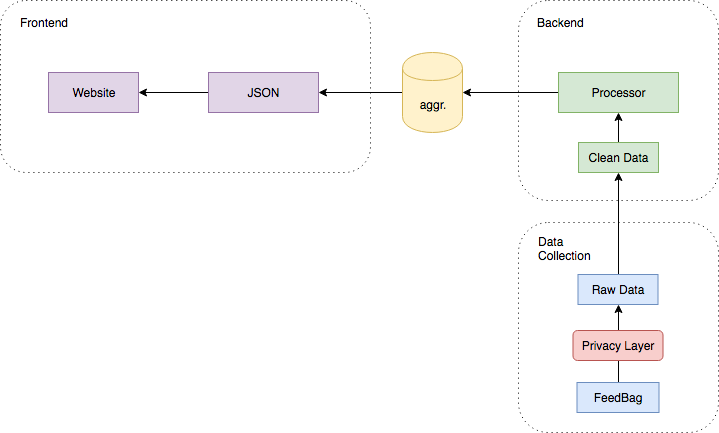
\includegraphics[width=\linewidth]{images/master_project_structure_v2.png}
  \caption{Structure overview}
  \label{fig:struct}
\end{figure}

\subsection{Criteria for success}
\subsection{Method of work}
\subsection{Quality management}
\subsubsection{Documentation}
\subsubsection{Validation steps}

\section{Plan with Milestone}
\subsection{Project steps}
\begin{figure}
  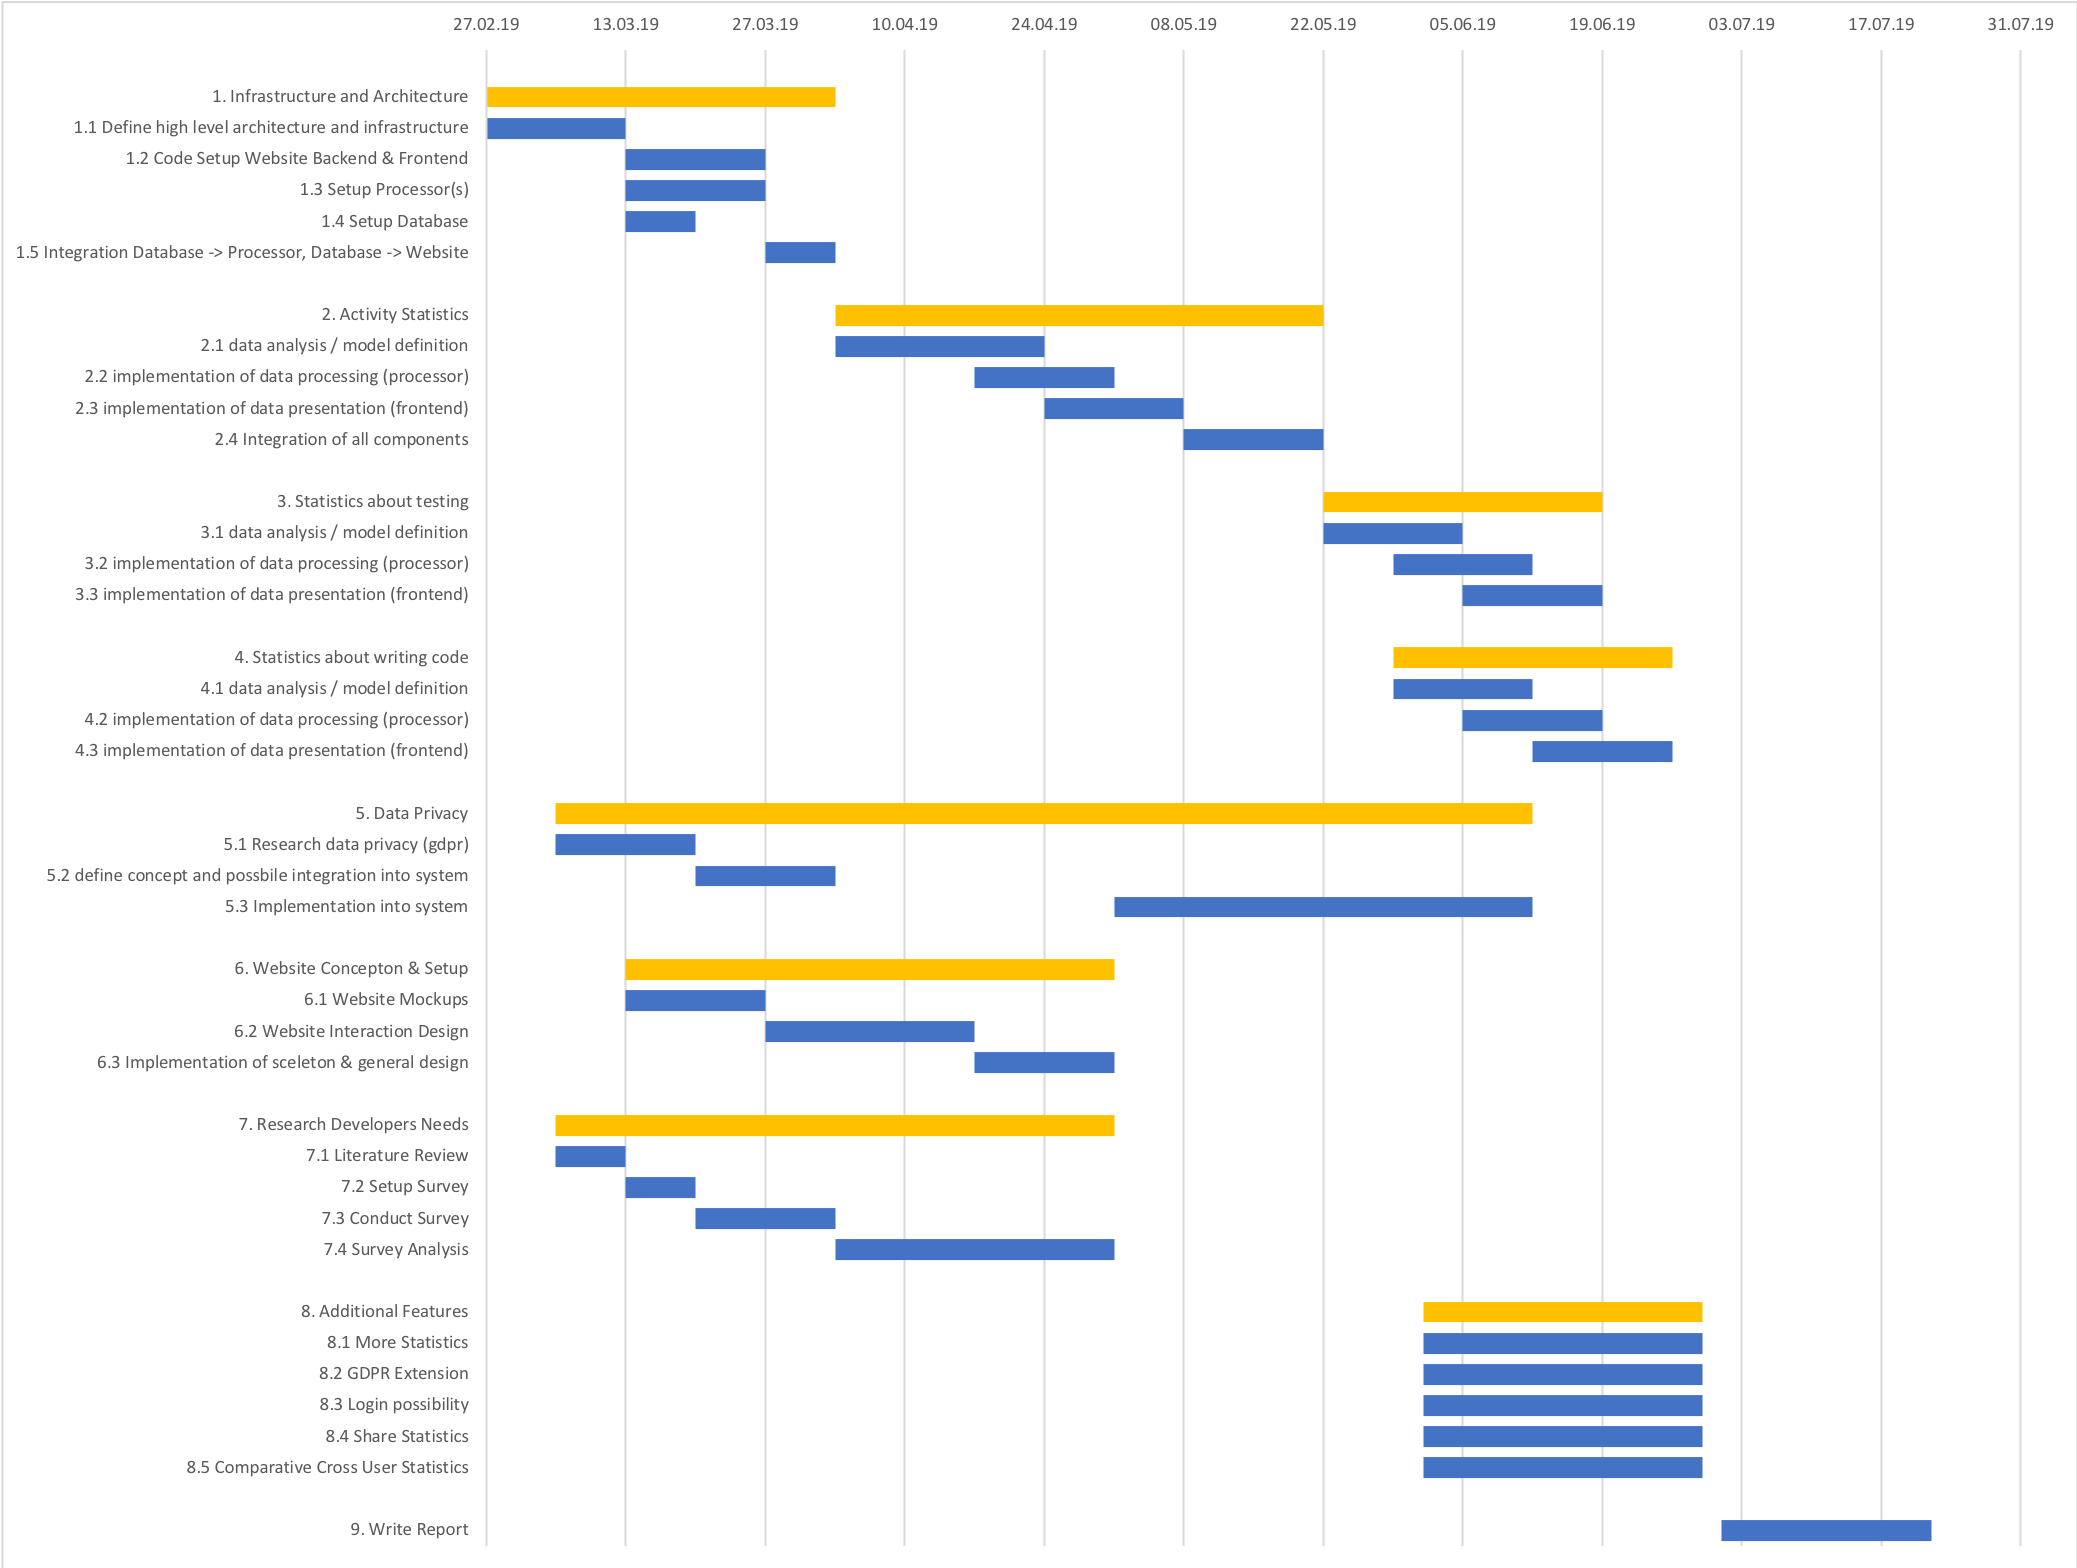
\includegraphics[width=\linewidth]{images/project_structure.png}
  \caption{Gantt chart of project deliverables}
  \label{fig:gantt}
\end{figure}

Our plan on what milestone we want to achieve to which time is shown as a gantt chart in Figure \ref{fig:gantt}.

\subsubsection{Infrastructure and Architecture}
First, we have to define a high level architecture and infrastructure for our system (1.1). We can only start implementing when the general structure of our system is set. In a second step, we define the structure for the individual parts and set up the website (with a backend and frontend part, (1.2)). At the same time, we plan to set up the processor(s) and database (1.3, 1.4). These two steps include a precise definition of the architecture and structure of the processor. The implementation follows afterwards. Lastly, the connection between the database and the processor is established as well as the connection between the database and the website (1.5).

\subsubsection{Activity Statistics}
The activity statistics track the users activities which consist of two states: The user is active (the IDE is open) and the user is inactive (the IDE is closed). In the active state, there are four more substates: Debugging, testing, producing code and exploring. These states are used to create a timeline which shows how much time the user spends on the individual states. Furthermore, we plan to create a pie chart which tracks the same data and represents it for certain time intervals, e.g. last week or last month.

To achieve this goal, we will have to decide how we would like to display the timeline and pie chart and how we are going to calculate the measures. A thorough data analysis and a model definition is essential for this task (2.1). In a later step, we will implement the calculations in the data processing part (processor) (2.2) and the visualisations in the frontend part (2.3). In the end, we will integrate all parts together (2.4). There should also exist a possibility to ​view the data generally or solution specific.

\subsubsection{Statistics about testing}
We plan to track information about testing: Number of written tests, number of executed tests, number of fixed tests and number of deleted tests. We are going to show this information on a timeline as well to inform the user how his behaviour has changed over time.

To achieve this goal, we will have to decide how we would like to display the timeline and how we are going to calculate the measures. A thorough data analysis and a model definition is essential for this task (3.1). In a later step, we will implement the calculations in the data processing part (processor) (3.2) and the visualisations in the frontend part (3.3). There should also exist a possibility to ​view the data generally or solution specific.

\subsubsection{Statistics about writing code}
Additionally, we plan to track information about the coding behaviour of users. These consist of the aggregated number of commits, the ​churn code-lines (+/-) (absolute sum of code-lines), the number of executions/builds and the build times. Like before, we would like to create a timeline which will give the users the chance to analyse their coding behaviour over time.

To achieve this goal, we will have to decide how we would like to display the timeline and how we are going to calculate the measures. A thorough data analysis and a model definition is essential or this task (4.1). In a later step, we will implement the calculations in the data processing part (processor) (4.2) and the visualisations in the frontend part (4.3). There should also exist a possibility to ​view the data generally or solution specific.

\subsubsection{Data privacy}
A new privacy concept has long been desired and with GDPR now being in effect, a new concept (including its implementation) is required. This requires research into the current interpretation of GDPR (5.1) and related laws, as well as the definition and implementation of the concept (5.2). Since the law only specifies a minimum of user control, there is a huge space of additional possibilities to give the user even more control (5.3).

\subsubsection{Website conception and setup}
Before actually displaying information, a lot has to be done concerning the website. We will experiment with various looks and feels, culminating in a mockup of the website (6.1), followed by a more detailed interaction design (6.2). With that, a skeleton implementation is possible and will be done before the implementation of the first metrics (6.3), such that the metrics display does not interfere with any other design task.

\subsubsection{Research developers needs}
This stage consists of four smaller tasks: Literature review (7.1), setting up a survey (7.2), conducting a survey (7.3) and doing a survey analysis (7.4). First, we have to research what has already been done in the field of useful coding-behaviour statistics. The knowledge gained in this step will be further used to set up a survey. The goal of this survey is to confirm our findings from the literature review and to spot other useful statistics we could use in our project. When we conduct the survey, we will distribute them to working software developers. In the end we will evaluate the survey results and use the findings to (if necessary) adapt our minimal features (see section 3., 4. and 5.) and design new additional features.

\subsubsection{Additional features}
With the time that is left at the end, we add additional features. What those are exactly is to be determined in the research part, but will resemble the following examples: Additional user control over their data (8.2), user accounts (8.3) and the possibility to remove your uploaded data, new metrics (8.1) (an example of such possible metrics is listed in Figure 2 in Meyer et al.’s paper [1, page 5]), enhanced metrics trend analysis (8.5), possibility to share ones statistics (8.4) or more control over the displayed data.

\subsubsection{Write report}
The last stage in our project consists of writing a report. We will describe all our working steps and results, analyse them and draw a conclusion in the end.

\subsection{Tentative schedule}

\section{Incremental Processing}
\begin{itemize}
\item 2018: Efficient finer-grained incremental processing with MapReduce for big data
\begin{itemize}
\item Most logging data is immutable in
\item More complicated: Also support modifying data
\item Difficult tradeoff: How big do we make the chunks? Big = lots to update, even with little new data, Small = too hard to search through all chunks
\item Incremental processing can save 85\%+ of processing time
\item Overview over existing incremental systems
\end{itemize}
\item 2013: large-scale incremental processing with mapreduce (HadUP)
\begin{itemize}
\item Current approaches are usually only for Big Data
\item Typical for incremental processing: deltas are much smaller than complete data
\item Common problem: small input change affects a lot of output (eg with PageRank)
\item Many approaces use memoization of intermediary results
\end{itemize}
\end{itemize}

%\nocite{Zobel04-writing, Strunk00-style}

\bibliographystyle{abbrv}
\bibliography{project_plan}

\end{document}
